\section{Multimodal Evidence Processing}
\subsection{Technical acquisition and derivatives}
Multimodal processing begins with local file identity and technical readability, not scene interpretation. \code{media_pipeline.py} streams SHA-256 calculation, probes media, and can perform strict full-file FFmpeg decoding. The separate video runner adapts downloaded archive manifests, validates local files, creates audio and sampled-frame derivatives, and optionally invokes OCR and ASR. Cache reuse depends on content, parameters, model/configuration and code fingerprints. Atomic writes and stat checks reduce accidental reuse of incomplete outputs. These are implemented engineering controls rather than a claim of forensic authenticity certification.

\begin{figure}[tbp]
\centering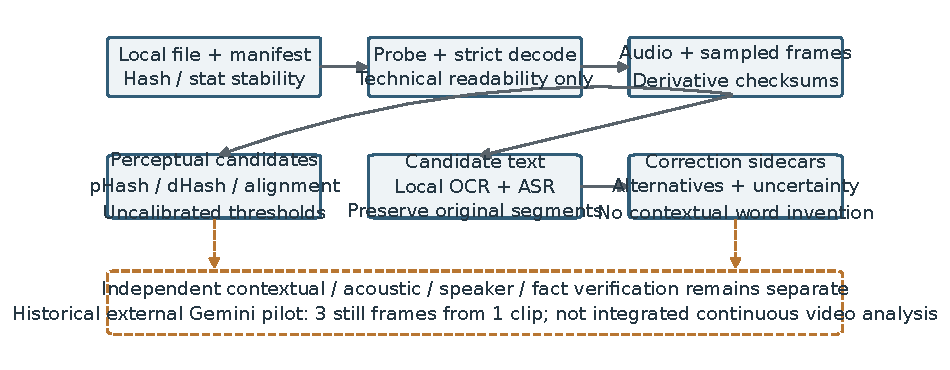
\includegraphics[width=\linewidth]{multimodal_pipeline.pdf}
\caption{Implemented local multimodal pipeline. Technical processing produces inspectable candidate observations. Independent acoustic, contextual, identity and event verification are separate tasks; the historical external three-keyframe Gemini pilot is not part of this automated runner.}
\label{fig:media}
\end{figure}

Sampled frame comparison combines a 63-bit low-frequency DCT perceptual hash and a 64-bit horizontal difference hash. It evaluates full, border-cropped and center-cropped variants, including horizontal mirrors, and excludes low-information frames. The default candidate rule uses Hamming limits of 10 and 12, at least .6 temporally consistent coverage of the shorter analyzed window, three distinct matching frames and hashes, and a two-second span. Nearest-frame offsets and their median deviation describe relative sequence alignment. These exploratory thresholds are not calibrated match probabilities. Similar overlays, static scenes and selection effects can produce false positives; sparse sampling, edits and cropping can produce false negatives. Neither a match nor a nonmatch establishes recording location, event identity, copy direction, or authenticity.

\subsection{Candidate speech and text}
The optional text path uses Tesseract OCR and faster-whisper ASR. OCR outputs word boxes and timestamps linked to frames; ASR outputs timed text segments. Tesseract's established OCR architecture and Whisper's multilingual training provide useful extraction foundations \citep{smith2007tesseract,radford2023whisper}. Their published results do not quantify performance of the exact converted models on Social's Ukrainian, Russian, mixed-language or noisy recordings. Faster-whisper's runtime and decoding settings also need explicit versioning \citep{systran2026faster}.

Historical bulk receipts name CPU/int8 \code{Systran/faster-whisper-small}, revision \code{536b0662742c02347bc0e980a01041f333bce120}, with faster-whisper 1.1.0. A selected seven-asset second pass used \code{mobiuslabsgmbh/faster-whisper-large-v3-turbo}, revision \code{0a363e9161cbc7ed1431c9597a8ceaf0c4f78fcf}. This selection is not a controlled corpus-wide model comparison. Original and alternative text are retained as correction sidecars; ten lexical candidates in that review remain \code{quote_safe=false}. Plausible contextual wording is insufficient grounds for silently filling inaudible speech.

Quotation safety has several separate requirements: text must match the audio, speaker identity must be justified if named, the quotation must preserve context, and factual assertions inside the quotation need their own evidence assessment. The 18-clip benchmark stores ten \code{quote_safe=true} flags, but an AI worker identifier accompanying a ``human acoustic listening'' field does not independently demonstrate a human listener. We report the supplied-reference error arithmetic and recorded flags, not independently verified quotation safety. Unexpectedly higher error in a nominal clean-speech stratum cannot establish a general noise effect: clips, terminology and reference construction differ, with only a few clips per stratum.

\subsection{External model feasibility versus integration}
A historical receipt describes a user-Agy Gemini 3.8 Flash pilot on three still frames from one 15.278-second clip. A full-video attempt was blocked, while the keyframe run returned candidate visual observations. This is feasibility evidence for an external tool invocation, without continuous-video, audio, geolocation, identity, truth or accuracy validation. The current Python runner contains no automatic Gemini/Agy call. Reported token counts are not a measured monetary cost, and outputs from another model are not independent corroboration of the scene.
